\newpage
\begin{flushleft}
  \textbf{\large 2 Обзор современных подходов к отслеживаю объектов на видеоизображениях}
\end{flushleft}
\refstepcounter{chapter}
\addcontentsline{toc}{chapter}{2 Обзор современных подходов к отслеживаю объектов на видеоизображениях}
В этой главе будут подобно рассмотрены следующие вещи:
\begin{itemize}
  \item[--] набор данных для сравнения различных алгоритмов друг с другом;
  \item[--] различные метрики, по которым проводится сравнение;
  \item[--] принцип работы и основные отличительные особенности выбранных алгоритмов. 
\end{itemize}
\section{Набор данных MOT17}
Набор данных MOTChallenge \cite{dendorfer2021motchallenge} является одним из наиболее популярных в области для сравнения между собой различных алгоритмов отслеживания нескольких объектов на видеоизображениях одновременно. 
Со дня своего появления он быстро обрел статус стандарта индустрии. 

Бенчмарк MOT17 был выпущен в 2017 году и является идейным наследником более ранних версий -- MOT15 и MOT16. В ходе этого развития авторами был исправлен ряд проблем старых версий:
\begin{itemize}
    \item[--] с развитием технологии отслеживания объектов на изображении MOT15 стал слишком простым для современных методов. MOT16 начал включать в себя ряд новых видео, где траектории объектов чаще пересекаются друг с другом, условия освещения более разнообразны, а средняя плотность объектов на изображении увеличилась в три раза;
    \item[--] MOT17 решает другую важную проблему -- уточняет разметку набора данных, так как в предыдущей версии нередко встречались ошибки. 
\end{itemize}

В итоге MOT17 включается в себя 14 различных видео общей протяженностью порядка 4 минут. Все они представляют из себя различные записи с уличных камер, на которых пешеходы перемещаются по тротуарам, площадям, торговым центрах. 
В наборе данных представлены различные ракурсы: как видео с подвижной камерой снятые человеком, находящимся в толпе, так и сделанные с возвышенности статично, например, камерой наблюдения.

На рисунках \ref{fig:mot_1}-\ref{fig:mot_3} приведены примеры изображений из бенчмарка.

\begin{figure}[ht]
    \centering
    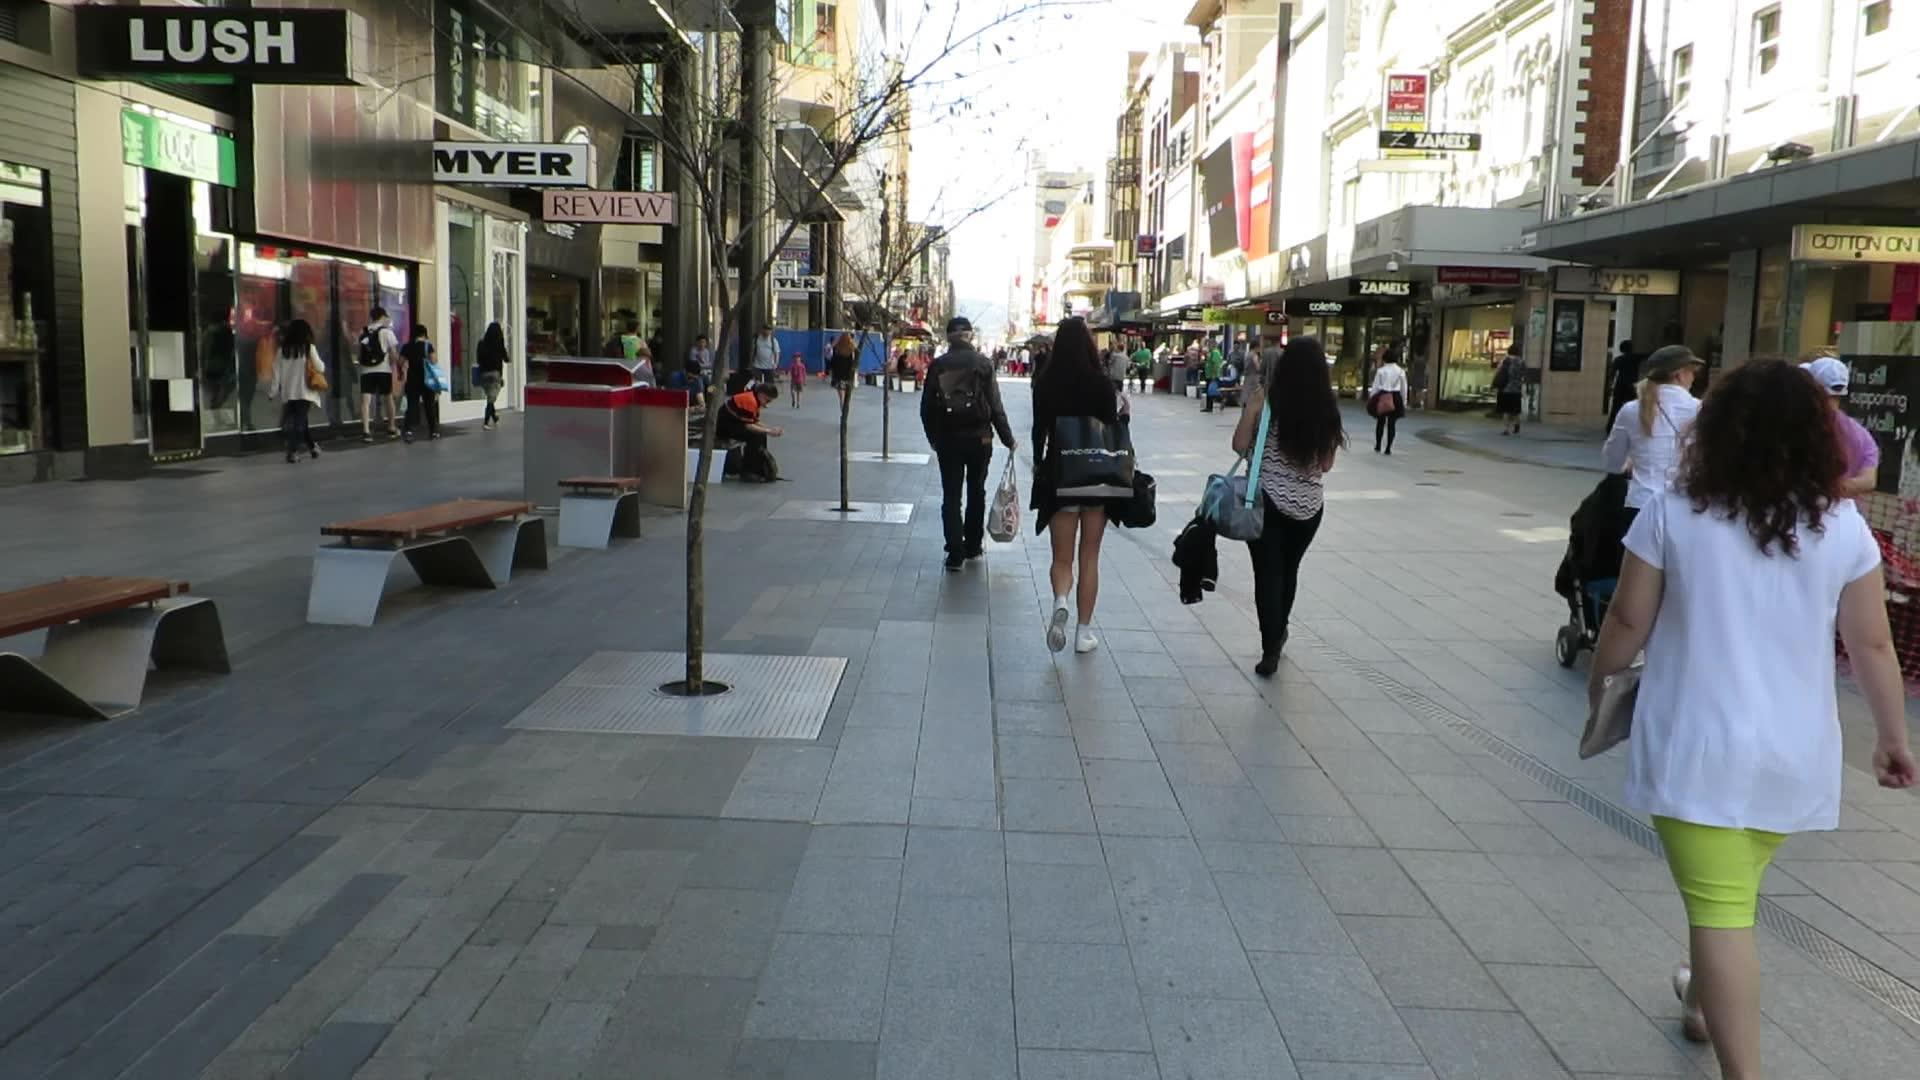
\includegraphics[width=0.7\textwidth]{review/MOT17_1}
    \caption{Пример изображения из набора данных MOT17 (приводится по \cite{dendorfer2021motchallenge}, страница 850, рисунок 3).}
    \label{fig:mot_1}
\end{figure}

\begin{figure}[ht]
    \centering
    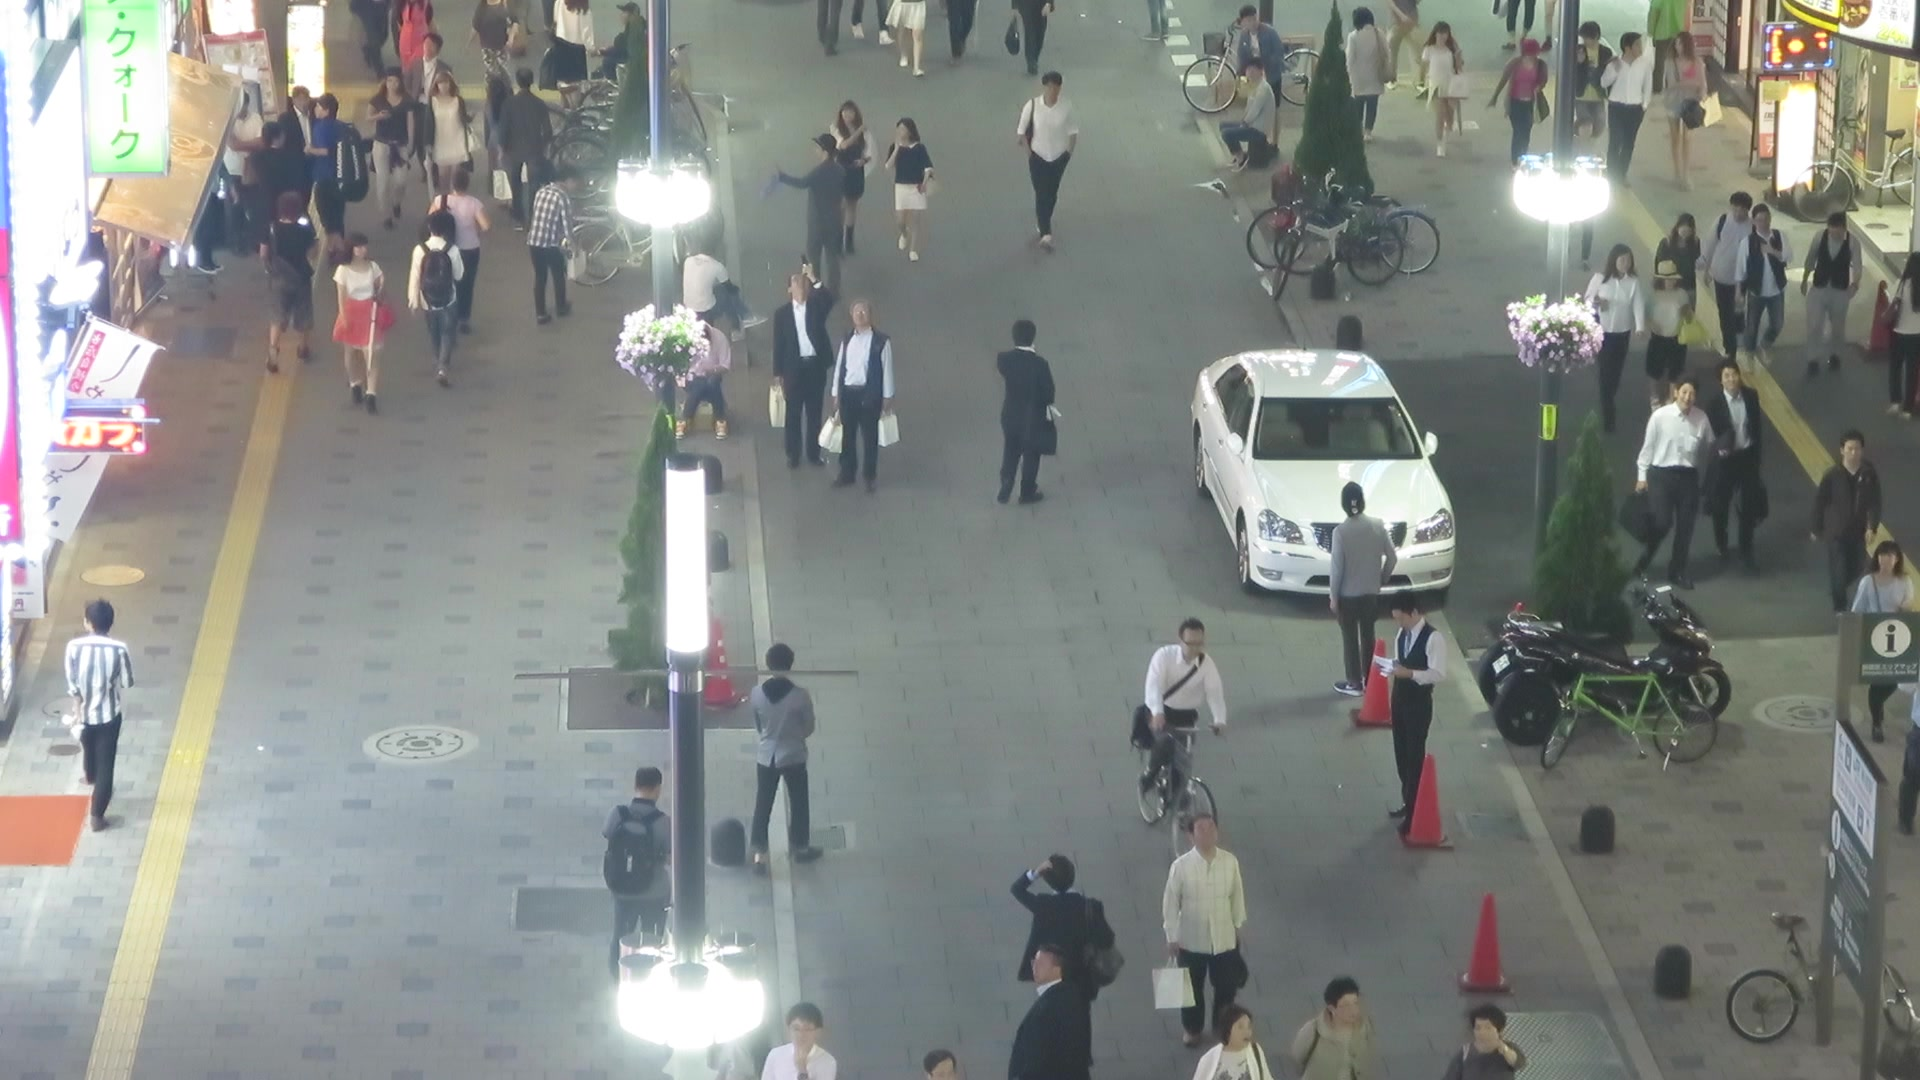
\includegraphics[width=0.7\textwidth]{review/MOT17_2}
    \caption{Пример изображения из набора данных MOT17 (приводится по \cite{dendorfer2021motchallenge}, страница 850, рисунок 3).}
    \label{fig:mot_2}
\end{figure}

\begin{figure}[ht]
    \centering
    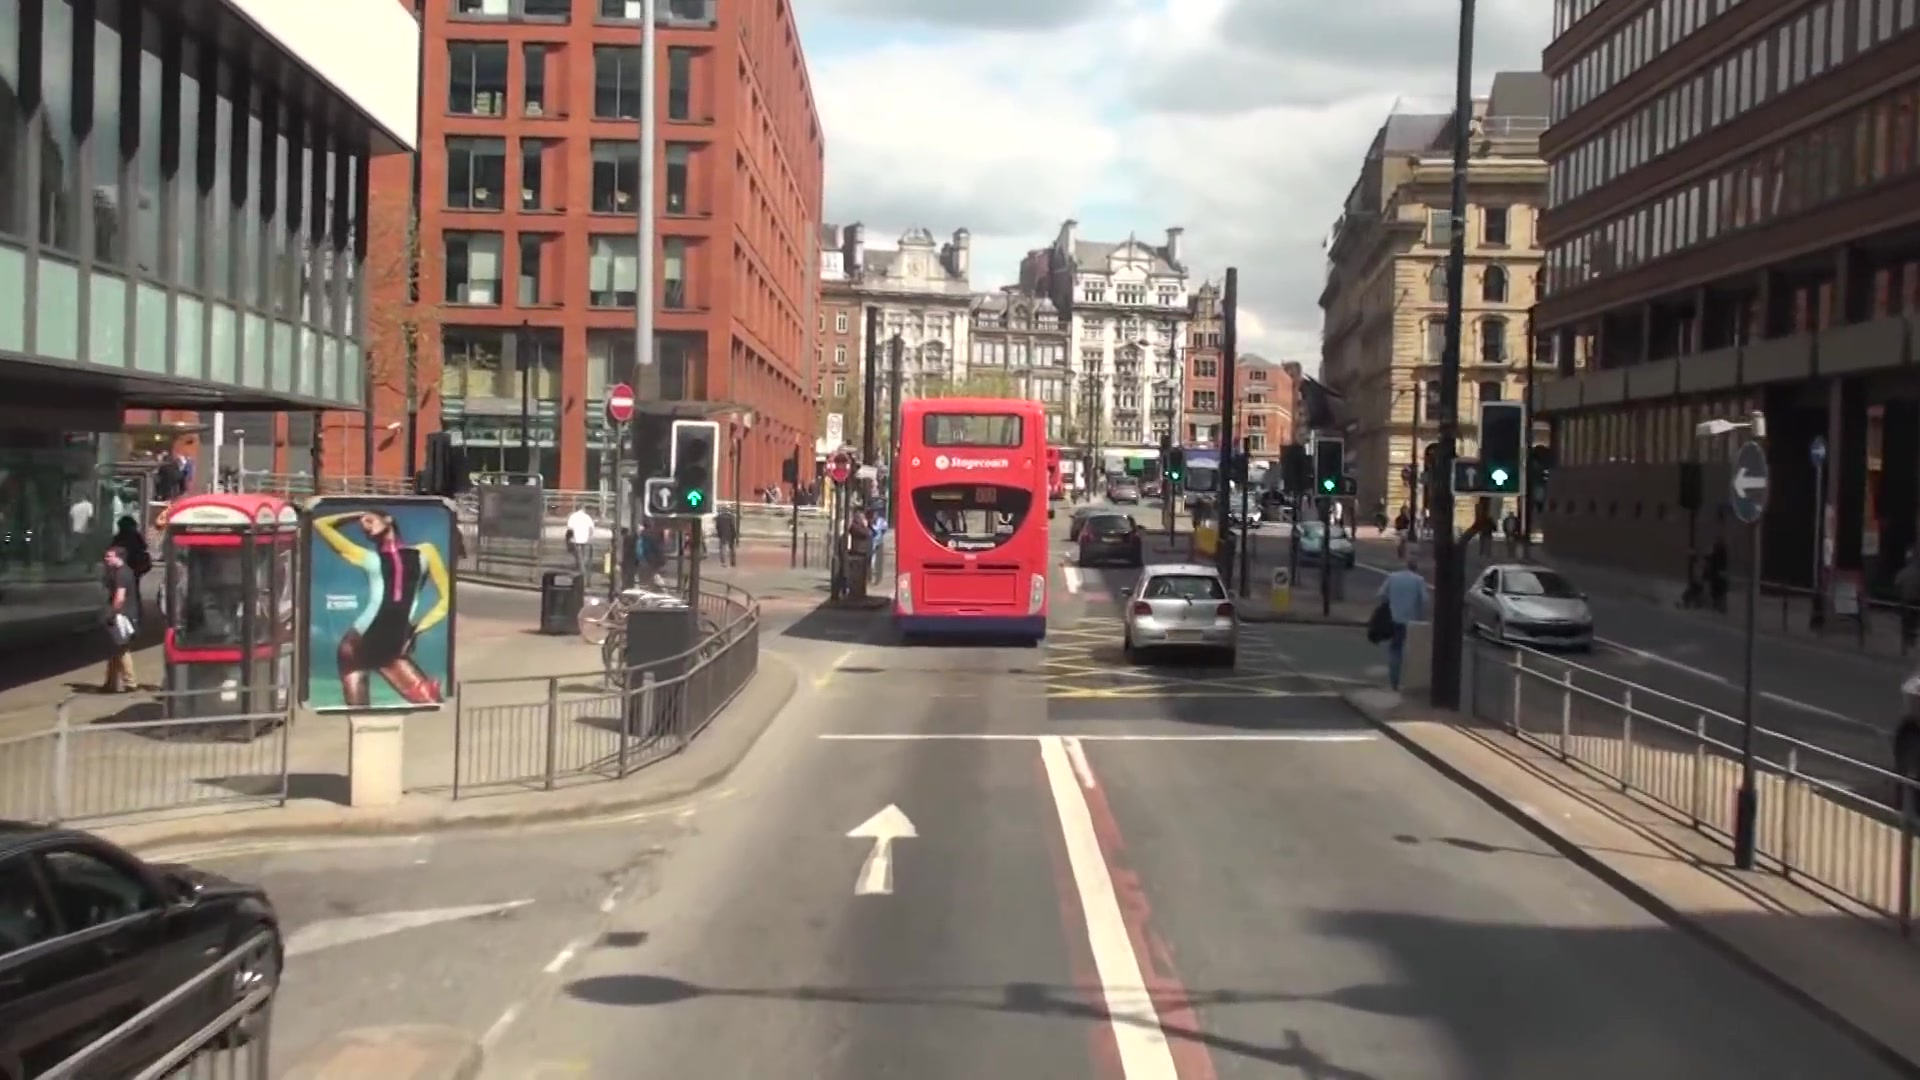
\includegraphics[width=0.7\textwidth]{review/MOT17_3}
    \caption{Пример изображения c из набора данных MOT17(приводится по \cite{dendorfer2021motchallenge}, страница 850, рисунок 3).}
    \label{fig:mot_3}
\end{figure}

\FloatBarrier
\section{Метрики для оценивания}
В этом разделе разбираются основные метрики для оценивания качества отслеживания объектов на видеоизображениях.
\subsection{Метрика MOTA}
Метрика МОТА\cite{bernardin2008evaluating} (англ. Multiple Object Tracking Accuracy -- точность отслеживания нескольких объектов) была предложена еще в 2008 году и является старейшей из всех используемых в работе. 
Ее авторы ставили целью создать критерий, который позволит оценивать точность выполнения задачи слежения. 
Подчеркивается важность способности метрики учитывать постоянство идентификации, точность оценки положения объекта и итоговой траектории.
Более того, был сделан акцент на минимизации параметров, а также интуитивной понятности для человека и применимости для задач слежения в любой постановке.

В итоге был предложен следующий способ вычисления 
\begin{equation}
    \text{MOTA} = 1 - \frac{\sum_{t=0}^{T}(\text{FP} + \text{FN} + \text{IDSW})}{\sum_{t=0}^{T}g_t},
    \label{eq:mota}
\end{equation}
где FP -- количество неверно найденных объектов, которые на самом деле не были отмечены на изображении при разметке; FN -- количество объектов, которые были отмечены при разметке, но не были найдены алгоритмом на изображении; 
IDSW -- сколько найденных ранее объектов не были правильно реидентифицированы и получили новый уникальный идентификационный номер, \(g_t\) -- общее количество объектов, отмеченных при разметке на кадре.
Из формулы \ref{eq:mota} видно -- чем больше показатель метрики, тем лучше справляется алгоритм.

Существует критика метрики MOTА, связанная с суммированием ошибок разного рода без какой-либо их предобработки, % \cite{dendorfer2021motchallenge}, 
а также плохой репрезентацией при отслеживании с использованием нескольких камер. % \cite{ristani2016performance}. 
Тем не менее, MOTA используется практически в каждом исследовании по теме и на практике доказала свою состоятельность в оценивании качества отслеживания объектов на видеоизображениях. Именно поэтому было принято решение включить ее в качестве критерия для сравнения методов в данной работе.
\subsection{Метрика IDF1}
Метрика IDF1 \cite{ristani2016performance} рекомендована для анализа производительности трекера в качестве дополнительно в связи с некоторым недостатками MOTA.

Авторы считали, что основная проблема других оценок -- арифметические операции с разнородными ошибками, которые могут оказывать влияние на интерпретируемость полученного результата. В общем, они оценивали вероятность появления ошибок идентификации и детектирования в каждый момент времени, а не точность итоговых траекторий у каждого объекта. 

Предложенная метрика IDF1 фокусировалась на оценке того, насколько качественно и долго трекер сохраняет идентичности объектов. Для этого, полученные с помощью трекера объекты, их идентичности и итоговые траектории сопоставляются с размеченными на основе методов графовой оптимизации, благодаря чему размеченные траектории сопоставляются с полученными на основе минимизации ошибки. Получившаяся оценка является более репрезентативной с точки зрения отслеживания конкретного объекта, так как оценивает именно задачу сохранения идентификации и точности итоговых траекторий.  
При этом у метрики есть и свои недостатки, поэтому авторы позиционирует ее как дополнительную для более комплексной оценки. 

Метрики IDF1 представляет из себя
\begin{equation}
    \label{eq:idf1}
    \text{IDF1} = \frac{2 \text{IDTP}}{2\text{IDTP} + \text{IDFP} + \text{IDFN}},
\end{equation}
где IDTP -- количество верно идентификационных отслеживаемых объектов; IDFN -- количество ненайденных объектов, которые были в разметке, но которым не были сопоставлены траектории; IDFP -- количество ложных срабатываний, когда был найден несуществующий объект. 
Расчет всех этих значений происходит после упомянутого ранее процесса сопоставления полученных траекторий с размеченными на основе оптимизации графа. 

% Полученная оценка является ед

В итоге, благодаря оценке с точки зрения качества сохранения присвоенных ранее идентификаций, метрика IDF1 является отличным дополнением для MOTA и была выбрана для учета в сравнении методов отслеживания объектов на видеоизображении в рамках данной работы.
\subsection{Метрика HOTA}
\cite{luiten2021hota}

\section{Обзор существующих алгоритмов}
В данном разделе разбирается принцип работы выбранных для исследования алгоритмов.
% Тут будут \cite{maggiolino2023deep, stadler2023improved}.
\subsection{Алгоритм ByteTrack}
Алгоритм ByteTrack \cite{zhang2022bytetrack} был представлен в 2022 году и сразу же завоевал первые позиции по качеству отслеживания объектов на изображениях на основе метрик MOTA, HOTA и IDF1.
До представления этого алгоритма, методы в основном основывались на работе только на показаниях детектора с высокой степенью уверенностью. Авторы же предложили способ получить преимущество, используя так же показания, в которых детектор не очень уверен.

На вход алгоритма поступают:
\begin{itemize}
    \item[--] видеоизображения, на которых предстоит провести отслеживание объектов;
    \item[--] детектор, который будет проводить детектирование объектов интересов;
    \item[--] граничная степень уверенности детектора \(\tau\). 
\end{itemize}
Выходом алгоритма являются получившиеся траектории. 

В ходе своей работы алгоритм сначала инициализирует массив траекторий для каждого найденного объекта. 
Затем в цикле для каждого кадра он получает набор пар область интереса-степень уверенности от детектора.
Полученные пары разбиваются на две группы: с высокой степенью уверенности большей \(\tau\) и с низкой. 
После этого для ранее найденных траекторий с помощью фильтра Калмана строится догадка об их положение на новом кадре.

Теперь начитается первый этап сопоставления. Для каждого объекта из группы с высокой степенью уверенности алгоритм подбирает близкую траекторию на основе метрики похожести. В ее роли может выступать как IoU (англ. Intersection over Union -- отношение площади пересечения к площади объединения двух объектов), так и ReID модель. 

На втором этапе сопоставления, для оставшихся траекторий, которым не нашлось объекта на первом этапе, производится попытка сопоставить объект из группы с низкой степенью уверености. На этом этапе рекомендуется использовать IoU, так как зачастую такие объекты смазаны или имеют какие-то перекрытия с другими, а потому ReID модели дают ненадежный результат.

Оставшиеся траектории помещаются в буфер потерянных траекторий. Если они находятся в этом буфере больше, чем какое-то количество итераций алгоритма (как правило 30 кадров или 1 секунда), то они удаляются из рассмотрения. Наличие это буфера критически важно, так как часто объекты бывают перекрыты полностью на короткий срок, во время которого сопоставление их траектории невозможно. Для таких траекторий происходит интерполяция их положения.

В работе на наборе данных MOT17 при использовании изображений размером \(800 \times 1440\) (оригинальный в наборе данных \(1080 \times 1920\)) получаются следующие показатели: MOTA -- 76.6; IDF1 -- 79.3; HOTA -- 63.1.

Для обучения сети детектора они использовали не только MOT17, но и CrowdHuman \cite{shao2018crowdhuman} с ETHZ \cite{ess2008mobile}.



\subsection{Алгоритм OC-SORT}
Алгоритм OC-SORT \cite{cao2023observation} был представлен чуть позже ByteTrack в 2022 году. 
В своей работе авторы работают над проблемой интерполяции траекторий. Более ранние подходы использовали только фильтр Калмана и опирались исключительно на его оценки в случае перекрытия или потери объекта. 
Это приводит к очевидным минусам таким как: 
\begin{itemize}
    \item[--] накопление шумов. Обычно скорость перемещения объектов на изображении всего несколько пикселей за кадр, а потому от кадра к кадру она может меняться в разы;
    \item[--] в случае нелинейного движения линейная аппроксимация также приводит к большим ошибкам на продолжительных отрезках времени.
\end{itemize}
Эти недостатки не критичны в том случае, когда потеря случается на короткий промежуток времени. Однако, если использовать такую оценку на протяжении десятка кадров без обновления фильтра Калмана, то накопленная ошибка будет уже значительна и не позволит сопоставить вновь найденный объект с его изначальной траекторией.
Авторы предлагают избежать этих проблем через смену подхода оценки на опирающийся больше на наблюдения. 

Первая из них решается благодаря ORU (англ. Observation-Centric Re-Update -- переобновление на основе наблюдений). После удачного сопоставления траектории с объектом после периода потери из поля зрения предлагается откатить состояние фильтра до того, что было в момент потери. После этого фильтр обновляют, подавая ему на вход виртуальную траекторию от точки потери до точки нахождения. Благодаря этому удается нивелировать ошибку состояния фильтра, накопленную при его слепом обновлении во время потери.

Второй способ, использующийся в работе -- OCM (англ. Observation-Centric Momentum -- момент на основе наблюдений). На основе последних нескольких показаний (как правило 3), распределенных через равные, не слишком маленькие промежутки времени, строится предположение траектории движения. После этого находится точка, которая меньше всего от него отклоняется. Этот способ лучше традиционного использования последних двух точек и линейной экстраполяции, так как меньше подвержен шумам. 

Полученный подход работает чуть лучше, чем ByteTrack: MOTA -- 78.0; IDF1 -- 77.5; HOTA -- 63.2.

\subsection{Алгоритм BoT-SORT}
BoT-SORT \cite{aharon2022bot} третий алгоритм, представленный в 2022 году. 
В своей работе авторы пишут, что алгоритмы, представленные раннее имеют множество недостатков.
Во-первых, фильтр Калмана используется для предсказания отношения ширины области интереса к ее высоте, что является причиной неточности оценки. 
Во-вторых, авторы утверждают, что в случае временной потери объекта из поля зрения реидентификация зачастую проваливается из-за неучтенного движения камеры. 
В-третьих, использование ReID моделей ведет к оптимизации метрики IDF1, в то время как IoU оптимизирует MOTA, поэтому существует вероятность улучшения производительности по обеим метрикам через введение нового способа определения похожести на основе двух этих. 

Для решения первой проблемы было предложено изменить классический для задачи отслеживания объектов на изображении вектор состояния фильтра Калмана 
\begin{equation}
    \label{eq:bot_old_kalman}
    x = [x_c, y_c, a, h, \dot x_c, \dot y_c, \dot a, \dot h]^T,
\end{equation}
где \((x_c, y_c)\) -- координаты области интереса, \(a\) -- отношение сторон области интереса, а \(h\) -- ее высота.
Вместо этого предложен вектор состояния
\begin{equation}
    \label{eq:bot_new_kalman}
    x = [x_c, y_c, w, h, \dot x_c, \dot y_c, \dot w, \dot h]^T,
\end{equation}
где \(w\) -- ширина области интереса. Авторы не очень понимают, почему это улучшает результат, но метрики растут. 

Для решения второй они добавляют использование алгоритма CMC (англ. Camera Motion Compensation -- компенсация движения камеры). При допущении, что объекты от кадра к кадру перемещаются по изображению несильно, данный подход значительно повышает робастность сопоставления траекторий и найденных объектов при нестабильном положении камеры в пространстве. 

Последняя проблема решается через комбинацию матриц близости IoU и косинусовых расстояний близости ReID модели. Для этого просто берется минимум для каждой пары объектов. 

Применение всех перечисленных подходов позволило добиться лучшего результата среди всех трекеров на тот момент: MOTA -- 78.5; IDF1 -- 82.1; HOTA -- 69.2.

\subsection{Алгоритм StrongSORT}
Алгоритм StrongSORT \cite{du2023strongsort} был представлен в 2023 году. 
Авторы поднимают вопрос отсутствия стандарта тестирования различных алгоритмов, в связи с чем иногда преимущество получают не те, 
которые работают эффективнее, а для которых был лучше обучен детектор.
Это затрудняет процесс объективного сравнения современных подходом между собой. 
Так же авторы утверждают, что если использовать старый алгоритм DeepSORT \cite{wojke2017deepsort}, но дооснастить его современными решениями, то получится конкурентноспособный подход. Свое желание актуализировать DeepSORT они мотивируют его легковесностью и эффективностью.

В итоге к алгоритму DeepSORT были добавлены:
\begin{itemize}
    \item[--] улучшенный экстрактор особенностей объектов;
    \item[--] компенсация движения камеры;
    \item[--] модифицированный для лучшей работы с шумами фильтр Калмана;
    \item[--] обновление особенностей объекта с помощью скользящего экспоненциального среднего;
    \item[--] реидентификация не только по внешнему виду, но и расстоянию Махаланобиса.
    % \item[--] 
\end{itemize}
Более того, авторы добавляют два новых алгоритма AFLink и GSI, которые позволяют качественнее обрабатывать моменты, когда объект теряется из кадра или перекрывается другими. 

Работа авторов демонстрирует эффективность модульного подхода в задаче отслеживания объектов на изображении. Алгоритм StrongSORT был получен наслаиванием друг на друга различных подходов, а так же добавлением нескольких новых методик.
Каждая из модификация дает прирост производительности в несколько пунктов, что в общей сумме повышает эффективность алгоритма и позволяет ему обойти все современные по показателям метрик: MOTA -- 77.1; IDF1 -- 82.3; HOTA -- 69.6.


\subsection{Алгоритм ImprAssOC}
Алгоритм ImprAsso \cite{stadler2023improved} также был представлен в 2023 году. 

Более ранние алгоритмы, как это было упомянуто в описании метода ByteTrack, делили объекты на две группы: с низкой и высокой степенью уверенности. 
Из-за этого объекты из группы с низкой степенью уверенности не могли быть сопоставлены с треками, объект которых потерян, а так же в целом приоритет всегда отдавался объектам с высокой. 
Авторы избегают этого, составляя матрицу расстояний сразу для всех объектов. Расстояния до объектов из группы с низкой степенью уверенности после этого нормализуются, чтобы быть одной размерности. 

Более того, авторы улучшают алгоритм ассоциации, потому что посчитали, что используемое в BoT-SORT взятие минимума из IoU и ReID не использует все доступные данные, а StrongSORT использует расстояние Махаланобиса, которое по их мнению дает только грубую оценку при высокой степени неизвестности.
Для этого, они комбинируют подходы и берут взвешенную сумму визуальных особенностей и расстояния до траектории, в случае если IoU больше какого-то значения, иначе просто присваивается максимальная степень непохожести.

Также авторы вводят новый подход для инициализации траектории. Раньше это либо происходило сразу для любого найденного объекта, что провоцировало создание лишних траекторий для FP результатов детектирования, либо инициализировали траекторию, если объект был найден n раз подряд, что искусственно создавало кадры, на которых объект найден, но еще не отслеживается. 
Суть подхода заключается в том, чтобы откинуть все FP объекты. Для всех несопоставленных с траекторией объектов вычисляется IoU с сопоставленными. Если оно больше какого-то граничного значения, то результат детектирования признается дубликатом и отбрасывается. 

Для обучения сети детектора используется MOT17, MOT20, CrowdHuman, ETH и CityPersons \cite{zhang2017citypersons}. Получены следующие показатели: MOTA -- 82.2; IDF1 -- 82.1; HOTA -- 66.4.

\subsection{Алгоритм Deep OC-SORT}
Алгоритм Deep OC-SORT \cite{maggiolino2023deep} последний из рассматриваемых в этой работе. 
Авторы решили совместить Deep-SORT и OC-Sort. Это чем-то похоже на StrongSORT, но со своими особенностями. 

Во-первых, предложен улучшенный алгоритм компенсации движения камеры. Так, фильтр Калмана, OCM и ORU получают на вход данные с компенсацией погрешностей, вызванных ее движением. 

Во-вторых, предложен улучшенный алгоритм скользящего экспоненциального среднего. Авторы по показателю уверенности в результате детектирования адаптивно меняют параметр, отвечающий за быстроту усреднения. Мотивация этого кроется в том, что если степень уверенности низкая, объект либо смазан, либо перекрыт другими объектами, а значит делать поправку на новые особенности стоит в меньшей степени.

В итоге полученный подход работает относительно лучше, чем OC-Sort: MOTA -- 75.6; IDF1 -- 79.2; HOTA -- 63.9. Хоть МОТА немного и упала, но IDF1 и HOTA выросли, что свидетельствует о лучшей работе с реидентификацией и особенностями объектов.


\section{Выводы по главе}
Во второй главе были рассмотрены:
\begin{itemize}
  \item[--] набор данных MOT17, на котором будет проводиться сравнение;
  \item[--] метрики, принцип вычисления каждой и концептуальные отличия полученных оценок;
  \item[--] разобран общий принцип работы методов отслеживания объектов на видеоизображениях, сравнение которых будет проведено в последующих главах.  
\end{itemize}